\documentclass[../NomeDocumento.tex]{subfiles}

\begin{document}
	
% NORME DI PROGETTO -> PROCESSI PRIMARI -> SVILUPPO

\section{Sviluppo}

\subsection{Scopo}

Il processo di sviluppo ha il fine di pianificare dettagliatamente e poi realizzare le attività che il gruppo di lavoro deve svolgere per fornire il prodotto richiesto dal capitolato.

\subsection{Descrizione}

Per una corretta implementazione di tale processo le aspettative sono le seguenti:

\begin{itemize}
	\item Realizzare un prodotto finale \glossario{conforme}{conforme} alle richieste della Proponente;
	\item Realizzare un prodotto finale soddisfacente i test di verifica;
	\item Realizzare un prodotto finale soddisfacente i test di validazione;
	\item Fissare gli obiettivi di \glossario{sviluppo}{sviluppo};
	\item Fissare i vincoli tecnologici;
	\item Fissare i vincoli di design.
\end{itemize}

\noindent Il processo di sviluppo si svolge in accordo con lo standard ISO/IEC 12207, pertanto si compone delle seguenti attività:

\begin{itemize}
	\item Analisi dei requisiti;
	\item Consolidamento dei requisiti e delle tecnologie;
	\item Progettazione;
	\item Codifica.
\end{itemize}

\subsection{Analisi dei Requisiti}

	\subsubsection{Scopo} 
	
	Gli \glossario{Analisti}{analista} devono individuare ed elencare i \glossario{requisiti}{requisito} del progetto da realizzare.
	
	\subsubsection{Descrizione}
	L'attività di Analisi deve:
	
	\begin{itemize}
		\item Descrivere il fine del progetto;
		\item Fissare le funzionalità e i requisiti richiesti dal committente.
	\end{itemize}

	\noindent Durante l’Analisi dei Requisiti gli \textit{Analisti} analizzano individualmente le varie fonti, quindi, a seguito di una riunione, si confrontano e stilano le varie liste di requisiti suddivise per importanza. Le fonti sono:
	 
	\begin{itemize}
		\item \textbf{Capitolato d’appalto:} requisiti emersi dall'analisi del documento fornito dalla Proponente;
		\item \textbf{Verbali esterni:} requisiti emersi a seguito di colloqui con i responsabili della Proponente;
		\item \textbf{Casi d'uso:} requisiti emersi a seguito di uno o più casi d’uso analizzati;
		\item \textbf{Tracciabilità Interna (TI):} requisiti emersi tramite discussioni ed incontri tra gli \textit{Analisti} del gruppo Graphite.
	\end{itemize}

	\subsubsection{Classificazione requisiti} 
	
	I requisiti devono essere suddivisi per importanza e classificati come segue:
	
	\begin{center}
		R[Importanza][Tipologia][Codice]
	\end{center}
		\begin{itemize}
			\item \textbf{Importanza:} Ogni requisito può appartenere solo ad una delle classi di Importanza elencate di seguito:
			\begin{itemize}
				\item \textbf{O (Requisito Obbligatorio):} requisito fondamentale per la corretta realizzazione del progetto;
				\item \textbf{D (Requisito Desiderabile):} requisito non fondamentale al progetto ma il cui soddisfacimento comporterebbe una maggiore completezza del prodotto;
				\item \textbf{F (Requisito Facoltativo):} requisito non richiesto per il corretto funzionamento del prodotto ma che se incluso arricchirebbe il progetto. Prima di soddisfare il requisito è necessaria un’analisi di tempi e costi per evitare ritardi nella consegna e/o costi superiori a quelli preventivati.
			\end{itemize}
			\item \textbf{Tipologia:} Di seguito sono riportate le tipologie di requisito:
			\begin{itemize}
				\item \textbf{V:} Identifica un \glossario{requisito di vincolo}{requisito di vincolo};
				\item \textbf{F:} Identifica un \glossario{requisito funzionale}{requisito funzionale};
				\item \textbf{P:} Identifica un \glossario{requisito prestazionale}{requisito prestazionale};
				\item \textbf{Q:} Identifica un \glossario{requisito di qualità}{requisito di qualita}.
			\end{itemize}
		\item \textbf{Codice:} Ogni requisito è formato da un codice numerico che lo indentifica in modo univoco.
		\end{itemize}
	
	\noindent Il codice stabilito secondo la convenzione precedente, una volta associato ad un requisito, non potrà cambiare nel tempo.
	
	\noindent Ciascun requisito dovrà inoltre essere accompagnato dalle sue fonti, dalle sue relazioni di dipendenza con altri requisiti e da una descrizione che ne specifichi lo scopo. Sarà inoltre indicata l'importanza.\\
	
	
	Esempio:
	\begin{figure}[h]
		\centering
		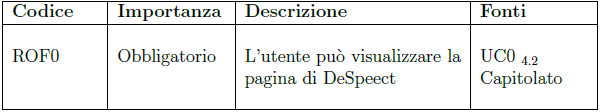
\includegraphics[width=0.7\linewidth]{img/esempio_tabella_requisiti}
		\label{fig:esempio di tabella dei requisiti}
		\caption{Esempio di tabella dei requisiti}
	\end{figure}
		
		
	\subsubsection{Classificazione casi d’uso} 
	
I \glossario{casi d'uso}{caso d'uso} verranno identificati nel seguente modo: 

\begin{center}
	UC[Codice padre]*.[Codice identificativo]
\end{center}

\begin{itemize}
	\item \textbf{Codice padre:} identifica il codice del caso d'uso da cui è stato generato il caso d'uso identificato, se non esiste il campo va tralasciato;
	\item \textbf{Codice identificativo:} identifica il caso d'uso univocamente.
\end{itemize}

	\noindent Ogni caso d'uso è inoltre definito secondo la seguente struttura:
\begin{itemize}
	\item \textbf{Attore Principale:} indica gli attori principali (ad esempio l'utente generico) del caso d'uso;
	\item \textbf{Attore Secondario:} indica gli attori secondari (ad esempio entità di autenticazione esterne) del caso d'uso;
	\item \textbf{Descrizione:} riporta una breve descrizione del caso d'uso;
	\item \textbf{Precondizione:} specifica le condizioni che sono identificate come vere prima del verificarsi degli eventi del caso d'uso;
	\item \textbf{Postcondizione:} specifica le condizioni che sono identificate come vere dopo il verificarsi degli eventi del caso d'uso;
	\item \textbf{Scenario Principale:} descrive il flusso degli eventi, a volte attraverso l'uso di una lista numerata o non, specificando i casi d'uso generati;
	\item \textbf{Scenari Alternativi:} specifica casi di errore o eventi non previsti nello scenario principale.
\end{itemize}

\subsection{Consolidamento dei requisiti e delle tecnologie}

	\subsubsection{Scopo} 
	
	In questa attività gli \textit{Analisti} devono affinare, ed eventualmente ampliare, i requisiti analizzati nel periodo di Analisi e, prima di iniziare l'attività di progettazione, i \textit{Progettisti} devono condurre un analisi delle tecnologie mirata alla scelta delle più appropiate ai fini del progetto, motivando e dimostrando la scelta mediante \glossario{Proof of Concept}{Proof of Concept}.
	
\subsection{Progettazione} 

	\subsubsection{Scopo} 

	L'attività di Progettazione deve obbligatoriamente precedere la produzione del software e consiste nel descrivere una soluzione del problema che sia soddisfacente per tutti gli \glossario{stakeholders}{stakeholders}. Essa serve a garantire che il prodotto sviluppato soddisfi le proprietà e i bisogni specificati nell'attività di analisi. 
	\subsubsection{Descrizione}
	
	La progettazione permette di:
	
	\begin{itemize}
		\item Costruire un’architettura logica del prodotto;
		\item Ottimizzare l’uso delle risorse;
		\item Garantire una determinata qualità del prodotto, perseguendo la \textit{correttezza per costruzione}: è questo il principio secondo il quale il software deve funzionare correttamente e soddisfare tutti i requisiti e i vincoli perché è stato progettato per farlo e per essere conforme ed \glossario{efficace}{efficacia}. Si trova in netta contrapposizione alla \textit{correttezza per
		correzione};
		\item Organizzare e dividere le parti del progetto in modo da poter ottenere componenti singole e facili da implementare attraverso la codifica. 
	\end{itemize}

	E' compito dei \textit{Progettisti} svolgere l'attività di Progettazione, definendo l'architettura logica del prodotto identificando componenti chiare, riusabili e coese, rimanendo nei costi fissati. L'architettura definita deve attenersi alle seguenti qualità:
	\begin{itemize}
		\item \textbf{Sufficienza:} soddisfare i requisiti definiti nel documento \textit{Analisi dei Requisiti};
		\item \textbf{Comprensibilità:} essere capita dagli stakeholders e quindi descritta in modo comprensibile, oltre ad essere tracciabile sui requisiti;
		\item \textbf{Modularità:} essere divisa in parti chiare e distinte, ognuna con la sua specifica funzione;
		\item \textbf{Robustezza:} essere in grado di gestire malfunzionamenti in modo da rimanere operativa di fronte a situazioni erronee improvvise;
		\item \textbf{Flessibilità:} permettere modifiche a costo contenuto nel caso in cui i requisiti dovessero evolversi o se ne dovessero aggiungere di nuovi;
		\item \textbf{Riusabilità:} essere costruita in modo da poter permettere il riutilizzo di alcune sue parti;
		\item \textbf{Efficienza:} soddisfare tutti i requisiti in modo tale da ridurre gli sprechi di tempo e spazio;
		\item \textbf{Affidabilità:} garantire che i servizi esposti siano sempre disponibili, ovvero svolgere i suoi compiti quando viene usata;
		\item \textbf{Disponibilità:} necessitare di tempo ridotto per la manutenzione in modo da garantire un servizio il più continuo possibile;
		\item \textbf{Sicurezza:} essere sicura rispetto ad intrusioni e malfunzionamenti;
		\item \textbf{Semplicità:} prediligere la semplicità, contenendo solo il necessario, rispetto ad una inutile complessità;
		\item \textbf{Incapsulazione:} fare in modo che l'interno delle componenti non sia visibile dall'esterno, seguendo il principio del \glossario{data hiding}{data hiding};
		\item \textbf{Coesione:} raggruppare le parti secondo l'obiettivo a cui concorrono, in modo da avere maggiore manutenibilità e riusabilità;
		\item \textbf{Basso accoppiamento:} non avere dipendenze indesiderabili.
	\end{itemize}
	
	%\subsubsection{Analisi delle tecnologie}
	%Prima di iniziare l'attività di progettazione, i \textit{Progettisti} devono condurre un analisi delle tecnologie mirata alla scelta delle più appropiate ai fini del progetto, motivando e dimostrando la scelta mediante \textit{Proof of Concept}.
	
	\subsubsection{Progettazione Architetturale}
	Finita l'attività di Analisi, è compito dei \textit{Progettisti} adottare opportune soluzioni progettuali a problemi ricorrenti. Tali soluzioni devono essere flessibili e consentire una certa libertà d'uso ai \textit{Programmatori}.
	
	\subsubsection{Progettazione in Dettaglio}
	Deve definire per ogni componente software il progetto della stessa e i relativi test.
%%	\subsubsection{UML 2.0}
%	
%		Al fine di rendere più chiare le scelte progettuali adottate e ridurre le possibili ambiguità, è necessario fare largo uso di vari tipi di diagrammi UML 2.0, tra cui:
	
%	\begin{itemize}
%		\item \textbf{Diagrammi delle classi:} definiscono relazioni, metodi e attributi di classi e tipi, astraendosi da un qualsiasi linguaggio di programmazione;
%		\item \textbf{Diagrammi dei \glossario{package}{package}:} illustrano raggruppamenti di classi che condividono la stessa causa di cambiamento e necessitano di essere riusate assieme;
%		\item \textbf{Diagrammi di sequenza:} servono a descrivere le interazioni che avvengono fra gli oggetti che devono implementare collettivamente un comportamento, rappresentando sequenze di azioni tramite scelte definite (ad esempio, una sequenza di invocazioni tra metodi);
%		\item \textbf{Diagrammi delle attività:} descrivono il flusso di operazioni di una attività (ad esempio un algoritmo), descrivendone la logica procedurale.
%	\end{itemize}
%
%	\noindent E' possibile inoltre fare uso di altre tipologie di diagrammi, come diagrammi delle componenti, di macchine a stati o di \glossario{deployment}{deployment}, se necessario.
	
	\subsection{Codifica}
	
	\subsubsection{Scopo}
	Nella seguente sezione sono riportate le norme da seguire durante la programmazione da parte dei \textit{Programmatori}. Lo scopo di queste norme consiste nel dare delle linee guida in modo tale che il codice risulti leggibile e facilmente analizzabile durante la fase di mantenimento, verifica e validazione, migliorando così la qualità del prodotto.

	\subsubsection{Descrizione}
	L'attività di codifica deve sviluppare il software e i test per le componenti descritti dalla progettazione in dettaglio assicurandosi che sia conforme a quanto definito. 
	
	\subsubsection{Norme di Codifica}
	Il gruppo aderisce alle \textit{GNU GCC Coding Conventions}, reperibili al seguente link:
	
	\begin{center}
		\url{https://gcc.gnu.org/codingconventions.html}
	\end{center}

	\noindent Segue quindi nelle successive sezioni una descrizione delle principali tra tali convenzioni di codifica.   
	
	\subsubsection{Linee di codice}
		Le linee di codice devono essere lunghe al massimo 80 colonne.
		
	\subsubsection{Nomi}
	\begin{itemize}
		\item \textbf{Univocità dei nomi:} classi, metodi e variabili devono avere un nome univoco e quanto più possibile esplicativo della loro funzione al fine di evitare ambiguità;
		
		\item \textbf{Macro:} i nomi delle macro devono essere tutti in maiuscolo;
		
		\item \textbf{Classi:} le classi iniziano sempre con una lettera maiuscola;
		
		\item \textbf{Metodi:} i nomi dei metodi iniziano con una lettera minuscola e se sono composti da più parole le successive devono iniziare con una lettera maiuscola. Le sigle e gli acronimi, all'interno dei nomi dei metodi, vengono trattate come parole;
		
		\item \textbf{Strutture:} quando le strutture e/o le classi hanno funzioni membro, i dati membro vanno nominati con il prefisso m\textunderscore , mentre i dati statici con il prefisso s\textunderscore;
		
		\item \textbf{Template:} i nomi dei parametri dei template devono usare \glossario{CamelCase}{CamelCase}, seguendo lo standard C++;
		
		\item \textbf{Altri nomi:} devono essere minuscoli e separati dal trattino basso.
	\end{itemize}	
	
	\subsubsection{Espressioni}
	\begin{center}
	\begin{tabular}{|l|c|c|}
		\hline
		Espressione&Convenzione adottata&Convenzione scorretta \\ \hline
		not logico&!x&! x \\ \hline
		complemento bit a bit&${\sim}x$&$\sim x$ \\ \hline
		meno unario&-x&- x \\ \hline
		conversione esplicita&(foo) x&(foo)x \\ \hline
		deferenziazione puntatore&*x&* x \\ \hline
	\end{tabular}
	\end{center}
	
	\subsubsection{Ereditarietà}
	Per quanto riguarda l'ereditarietà è necessario attenersi ai seguenti accorgimenti:
	\begin{itemize}
		\item È consentita l'ereditarietà singola;
		\item Deve essere utilizzata l'ereditarietà pubblica per l'interfaccia, cioè le relazioni \textit{"is-a"};
		\item Deve essere utilizzata l'ereditarietà privata e protetta per l'implementazione; 		
		\item Le gerarchie complesse devono essere evitate;
		\item L'ereditarietà multipla deve essere trattata con molta attenzione e nel caso venga usata deve essere scritta una documentazione particolarmente chiara dell'intera gerarchia. In generale, è preferibile non usarla.
	\end{itemize}
	
	\subsubsection{Definizioni}
	\begin{itemize}
		\item \textbf{Variabili:} le variabili devono essere definite nel momento del loro primo utilizzo. Possono essere definite e testate simultaneamente nelle espressioni di controllo;
		
		\item \textbf{Strutture:} la parola chiave \textit{struct} deve essere utilizzata solo per i \glossario{POD}{POD};
		
		\item \textbf{Classi:} Per la definizione di classe devono essere usate le seguenti regole:
		
		\begin{itemize}
			\item \textbf{Parola chiave:} la parola chiave \textit{class} deve essere utilizzata solo per i tipi non POD.
			\item \textbf{Indentazione:} metodi e campi dati membri della classe devono essere indentati di due spazi;
			\item \textbf{Definizione in singola riga:} se possibile, la classe deve essere definita su una singola riga, come nel seguente esempio:
			
			\begin{verbatim}
			class gnuclass: base {
			\end{verbatim}
			
			Se ciò non fosse possibile, si deve iniziare la lista delle classi base con i due punti dell'elenco all'inizio della riga successiva, come di seguito mostrato.
			
			\begin{verbatim}
			class a_rather_long_class_name
			: with_a_very_long_base_name, and_another_just_to_make_life_hard {
				...
			};
			\end{verbatim}
			
			Se l'elenco dovesse superare la lunghezza di una riga, si devono spostare le classi base in eccesso alla riga successiva con il rientro di due spazi, come illustrato nel seguente esempio:
			
			\begin{verbatim}
			class gnuclass
			: base1 <template_argument1>, base2 <template_argument1>,
			base3 <template_argument1>, base4 <template_argument1> {
				....
			};
			\end{verbatim}
		
			
			\item \textbf{Ordine degli elementi:} quando si definisce una classe, l'ordine in cui definire i suoi elementi (metodi o campi dati) deve essere il seguente:
			
			\begin{enumerate}
				\item Tipi pubblici;
				\item Tipi non pubblici;
				\item Costruttori pubblici;
				\item Distruttore pubblico;
				\item Metodi pubblici;
				\item Campi dati pubblici;
				\item Costruttori non pubblici;
				\item Distruttore non pubblico;
				\item Metodi non pubblici;
				\item Campi dati non pubblici.				
			\end{enumerate}
			
			Se vincoli semantici richiedessero un diverso ordine di dichiarazione, se deve cercare di minimizzare la potenziale confusione (per esempio attraverso appositi commenti al codice).
			
			\item \textbf{Apertura e chiusura} una definizione di classe deve essere aperta con una parentesi graffa sinistra in linea e chiusa con una parentesi graffa destra, punto e virgola, commento di chiusura facoltativo e una nuova riga, come illustrato nel seguente esempio:
			
			\begin{verbatim}
			class gnuclass: base {
			...
			}; // class gnuclass
			\end{verbatim}	
		\end{itemize}

	\item \textbf{Membri di una classe:} tutti i membri di una classe vanno definiti al di fuori della definizione della stessa, cioè non ci sono corpi di funzioni o inizializzatori di campi dati all'interno della definizione della classe. È inoltre necessario attenersi alle seguenti indicazioni:
	
	\begin{itemize}
		\item È preferibile scrivere l'intera definizione di un metodo su di una singola riga, come nel seguente esempio:
		
		\begin{verbatim}
		gnuclass::gnuclass () : base_class () { 
			...
		};
		\end{verbatim}
		
		Se ciò non fosse possibile, si deve iniziare la lista di inizializzazione con i due punti dell'elenco all'inizio della riga successiva, come di seguito mostrato.
		
		\begin{verbatim}
		gnuclass::gnuclass ()
		: base1 (), base2 (), member1 (), member2 (), member3 (), member4 () { 
			...
		};
		\end{verbatim}
		
		Se l'elenco dovesse superare la lunghezza di una riga, si devono spostare gli inizializzatori in eccesso alla riga successiva con il rientro di due spazi, come illustrato nel seguente esempio:
		
		\begin{verbatim}
		gnuclass::gnuclass ()
		: base1 (some_expression), base2 (another_expression),
		member1 (my_expressions_everywhere) { 
			...
		};
		\end{verbatim}
		
		\item Se il nome di una funzione è sufficientemente lungo da permettere che il primo parametro di funzione con il suo tipo superi 80 caratteri, deve apparire nella riga successiva preceduto da quattro spazi di indentazione, come illustrato nell'esempio seguente:
		
		\begin{verbatim}
		void
		very_long_class_name::very_long_function_name (
		very_long_type_name arg)
		{
		\end{verbatim}
		
		\item Se la somma delle lunghezze del qualificatore della classe e del nome della funzione supera le 80 colonne, la riga va interrotta per andare a capo con l'operatore \textit{"::"}, come illustrato nell'esempio seguente:.
		
		\begin{verbatim}
		void
		very_long_template_class_name <with, a, great, many, arguments>
		::very_long_function_name (
		very_long_type_name arg)
		{
		\end{verbatim}		
	\end{itemize}
	
	\end{itemize}
	
	\subsubsection{Costruttori} 
	Ogni costruttore deve inizializzare i membri dei dati nell'elenco di inizializzazione dei membri, piuttosto che nel corpo del costruttore.
		
	\subsubsection{Distruttori}
	Una classe con funzioni virtuali deve necessariamente avere un distruttore virtuale.
		
	\subsubsection{Conversioni} 
	I costruttori a singolo argomento devono essere sempre dichiarati esplicitamente.	Gli operatori di conversione devono essere il quanto più possibile evitati.
	
	\subsubsection{Overloading}
	\begin{itemize}
		\item \textbf{Overloading delle funzioni:} è consentito fare \glossario{overloading}{overloading} di funzioni. Non tuttavia è consigliato farlo per le funzioni virtuali;
		
		\item \textbf{Overloading degli operatori:} è consentito fare overloading degli operatori. L'overloading degli operatori, ad eccezione dell'operatore di chiamata, non deve essere utilizzato per implementazioni costose.
	\end{itemize}

	\subsubsection{Argomenti di default} 
	Gli argomenti di default sono un altro tipo di overloading di funzioni, per cui vi si applicano le medesime regole. Gli argomenti di default devono sempre essere valori POD, cioè non possono eseguire costruttori. Le funzioni virtuali non devono avere argomenti di default.
		
	\subsubsection{Funzioni inline}
	 Sono preferite funzioni non in linea, a meno che non si abbia prova che la versione in linea della stessa funzione sia significativamente più piccola o meno impattante sulle prestazioni.
	
	\subsubsection{Template} 
	Una dichiarazione che segue un elenco di parametri del template non dovrebbe avere indentazione aggiuntiva, ed è preferito il typename sulla classe nella lista di parametri del template. Per non gravare eccessivamente sulle prestazioni, si raccomanda di fare uso parsimonioso dei template.
	
	\subsubsection{Namespace} 
	I namespace sono incoraggiati, tutte le librerie separabili devono avere un unico namespace globale. I nomi delle directory annidate devono essere associati a namespace annidati quando possibile. I file header non devono avere direttive \textit{using}.
	
	\noindent Un namespace va aperto con il nome seguito da una parentesi graffa sinistra e una nuova riga e chiuso con una parentesi graffa destra, un commento di chiusura facoltativo e una nuova riga, come evidenziato nel seguente esempio:
	
	\begin{verbatim}
	namespace gnutool {
	...
	} // namespace gnutool
	\end{verbatim}
	
	\noindent Le definizioni all'interno del corpo di un namespace non sono indentate.
	
	\subsubsection{Extern} è preferito un blocco extern al posto di un qualificatore di dichiarazione.
	
	\noindent Un blocco extern va aperto e chiuso nel modo seguente:
	
	\begin{verbatim}
	extern "C" {
	...
	} // extern "C"
	\end{verbatim}
	
	\noindent Le definizioni all'interno del corpo di un blocco extern non sono indentate.
\end{document}